%%%%%%%%%%%%%%%%%%%%%%%%%%%% Huong dan su dung compiler %%%%%%%%%%%%%%%%%%%%%%%%
% Latex>biber>latex>makeglossary>latex> makeindex > latex > pdflatex > view-pdf%
%%%%%%%%%%%%%%%%%%%%%%%%%%%%%%%%%%%%%%%%%%%%%%%%%%%%%%%%%%%%%%%%%%%%%%%%%%%%%%%%

\documentclass[12pt,a4paper,reqno, oneside]{book}
\makeindex
\usepackage[utf8]{vietnam}
\usepackage{amsmath, amsthm, amssymb,latexsym,amscd,amsfonts,enumerate}
\usepackage[backend=biber,style=numeric,sorting=ynt,hyperref=auto,doi=true]{biblatex}
\addbibresource{thesis.bib}
\usepackage{stdclsdv}
\usepackage[]{tocbibind}
\usepackage[titletoc]{appendix}
\usepackage[hidelinks]{hyperref}
%%%%%%%%%%%%%%%%%%%%%%%%%%%%%%%% trang tri %%%%%%%%%%%%%%%%%%%%%%%%%%%%%%%%%%%%%
\setlength{\oddsidemargin}{0in}
\setlength{\textwidth}{6.in}
\setlength{\topmargin}{-0.5in}
\setlength{\textheight}{9.25in}
\renewcommand{\baselinestretch}{1.5}
\usepackage{color, fancyhdr, graphicx, wrapfig}
\usepackage{epstopdf}

\pagenumbering{roman}\pagestyle{plain}
\pagestyle{fancy}
\lhead{\it Tương tác lực giữa phân tử VP35 và dsRNA của virus Ebola}
\rhead{\it }
\lfoot{\it Nguyễn Hữu Quý Ngân} 			         
\rfoot{\it Theoretical Physic - HCMUS}
\renewcommand{\headrulewidth}{1,2pt} 			
\renewcommand{\footrulewidth}{1,2pt}   % Cái này là tiêu đề chạy

%%%%%%%%%%%%%%%%%%%%%%%%%%%% Figures and Table %%%%%%%%%%%%%%%%%%%%%%%%%%%%%%%%%
\usepackage{afterpage, caption, subcaption}

%%%%%%%%%%%%%%%%%%%%%%%%%%%% Tu dien viet tat %%%%%%%%%%%%%%%%%%%%%%%%%%%%%%%%%%

\usepackage{glossaries}
\makeglossaries
\setacronymstyle{long-short}
\newacronym{ebov}{EBOV}{virus Ebola}
\newacronym{zebov}{ZEBOV}{Zaire Ebola}
\newacronym{evd}{EVD}{Bệnh Ebola - Ebola Virus Disease -}
\newacronym{ehf}{EHF}{Sốt xuất huyết Ebola - Ebola Hemmohaegic Fever -}
\newacronym{md}{MD}{phương pháp động học phân tử - Molecular dynamics -}
\newacronym{smd}{SMD}{Steered Molecular Dynamcs}
\newacronym{dsrna}{dsRNA}{chuỗi kép RNA - double-strain RNA -}
\newacronym{iid}{IID}{Interferon Inhibitor Domain}
\newacronym{meta}{metadynamics}{metadynamcis}
\newacronym{amber}{amber99sb ff}{trường lực AMBER99SB}
\newacronym{gp}{GP}{Glycoprotein}
\newglossaryentry{ifn}
{
name={IFN},
description={Interferon (IFN) là một nhóm các protein tự nhiên được sản xuất bởi các tế bào của hệ miễn dịch ở hầu hết các động vật nhằm chống lại các tác nhân ngoại lai như virus, vi khuẩn, kí sinh trùng và tế bào ung thư.\cite{DeAndrea2002}},
%other options
}\newacronym{np}{NP}{Nucleoprotein}
\newglossaryentry{rig-i}
{
name={RIG-I},
description={retinoic acid-inducible gene 1 là một loại enzym có chức năng phát hiện chuỗi vật chất di truyền của các virus cúm A, virus Sendai, họ flavivirus (virus sốt xuất huyết, viêm não Nhật Bản,...). Tuy nhiên RIG-I không phát hiện được retrovirus hay virus có vật chất di truyền là DNA.\cite{Kato2008}},
%other options
}










\begin{document}

\newpage
\begin{titlepage}
\centerline{\bf ĐẠI HỌC QUỐC GIA TP.HCM}
\centerline{\bf TRƯỜNG ĐẠI HỌC KHOA HỌC TỰ NHIÊN}
\centerline{\bf KHOA VẬT LÝ-VẬT LÝ KỸ THUẬT}
\vspace*{1cm}
\centerline{KHÓA LUẬN TỐT NGHIỆP}
\centerline{Ngành: Vật lý Lý thuyết}
\vspace*{1cm}
\centerline{\bf Nguyễn Hữu Quý Ngân}
\vspace*{3cm}
\centerline{\Large\bf TƯƠNG TÁC LỰC GIỮA PHÂN TỬ VP35}
\vspace*{0.5cm}
\centerline{\Large\bf VÀ dsRNA CỦA VIRUS EBOLA}
\vspace*{4cm}
\centerline{\bf Người hướng dẫn: }
\centerline{\bf TS. Nguyễn Hà Hùng Chương}
\vfill
\centerline{\bf TP.HCM 07/2014}
\end{titlepage}

\pagestyle{plain}
%\input Loicamon

\cleardoublepage% \clearpage
\pagestyle{fancy}
\pagenumbering{roman}
\tableofcontents
\clearpage

\printglossaries
\addcontentsline{toc}{chapter}{Từ điển chú giải}
\clearpage

\newpage
\pagestyle{fancy}
\listoffigures



\newpage
\pagestyle{fancy}
\setcounter{page}{1}
\pagenumbering{arabic}
%%%%%%%%%%%%%%%%%%%     Loi mo dau       %%%%%%%%%%%%%%%%%%%%%%%%
%%%%%%%%%%%%%%%%%%%                      %%%%%%%%%%%%%%%%%%%%%%%%
\setcounter{chapter}{-1}
\chapter{Lời mở đầu}
\hspace{20pt}
	Đề tài tập trung vào việc phân tích tương tác của phân tử VP35 và \gls{dsrna} của virus Ebola (\gls{ebov}) nhằm đánh giá các amino acid có vai trò quan trọng trong tương tác giữa hai phân tử trên. Theo đó, kết quả của khóa luận kiểm tra những amino acid thứ 312 và 339 của VP35 đóng vai trò quan trọng trong tương tác VP35-dsRNA\cite{Leung2010}. Đồng thời tiên đoán đột biến amino acid thứ 282 từ Lysine thành Alanine (K282A) làm giảm khả năng liên kết giữa VP35 và \gls{dsrna}.
	
	Phương pháp được sử dụng là \gls{smd}. Mô hình phân tử nước được sử dụng là TIP-4P\cite{Horn2004} và \gls{amber}\cite{} trong quá trình mô phỏng động học.
	
	Đề tài gồm 4 chương:
	\begin{itemize}
	\item Chương 1: Bệnh Ebola, \gls{ebov} và sự cần thiết của việc nghiên cứu \gls{ebov}, quá trình \gls{ebov} sao chép và vai trò của protein VP35, một số phương án ngăn chặn \gls{ebov} và một số nghiên cứu gần đây.
	\item Chương 2: Các cấu hình của VP35 được khảo sát, \gls{md} và phần mềm, công cụ sử dụng để khảo sát tương tác giữa VP35 và \gls{dsrna}.
	\item Chương 3: Trình bày các kết quả thu được và thảo luận tương ứng.
	\item Chương 4: Các kết luận và hướng phát triển tiếp theo của đề tài.
	\end{itemize}

	Do thời gian thực hiện khóa luận không nhiều, kiến thức còn hạn chế nên khi làm đề tài không tránh khỏi những hạn chế và sai sót. Tác giả rất mong nhận được sự góp ý và những ý kiến phản biện của quý thầy cô và các bạn.
	\textrm{Xin chân thành cảm ơn!}
 


\newpage
\pagestyle{fancy}
%%%%%%%%%%%%%%%%%%%     Chuong 1       %%%%%%%%%%%%%%%%%%%%%%%%
%%%%%%%%%%%%%%%%%%%                    %%%%%%%%%%%%%%%%%%%%%%%%
\setcounter{chapter}{0}
\chapter{Tổng quan}
\hspace{18pt}
\section{Bệnh do Virus Ebola}
\hspace{18pt}
	\gls{evd} hay \gls{ehf} là bệnh truyền nhiễm trên động vật có vú gây bởi \glsentryfull{ebov}. Bệnh được phát hiện lần đầu năm 1976 tại Trung Phi\cite{}. Tỉ lệ tử vong nếu không được chữa trị lên đến 90\% ở chủng \gls{zebov}\cite{}. Đây là bệnh có tốc độ bùng phát cao và khó kiểm soát do Ebola có thể lây truyền qua nhiều động vật là vật chủ trung gian, đồng thời lây truyền qua tiếp xúc với dịch tiết từ cơ thể người bệnh\cite{}.
	
	\gls{evd} đặc biệt nguy hiểm và có khả năng xuất hiện ở các nước có khí hậu nhiệt đới, cận nhiệt\cite{}. Đồng thời, \gls{evd} lây truyền qua dơi ăn trái cây và các động vật như tinh tinh, khỉ, heo\cite{Kuhn2010}, nên khả năng xuất hiện ở Việt Nam là rất cao. Trong nhiều thập kỷ, việc tìm hiểu về \gls{ebov} được quan tâm nhiều khi vũ khí sinh học trở nên phát triển\cite{}.
	
\subsection{Các protein của \glsentrytext{ebov}}
\hspace{18pt}
	Cần biết rõ về các protein có trong \gls{ebov} để phác thảo được các phương án tấn công \gls{ebov} được nói đến ở mục tiếp theo.
	\Gls{ebov} thuộc họ Filoviridae, bộ Mononegravirale\cite{Kuhn2010}, tức là \gls{ebov} thuộc họ virus có vật chất di truyền RNA gram âm và có ???????????????????? .\Gls{ebov} được cấu tạo bởi 7 loại protein với các chức năng khác nhau\cite{}.
	\begin{itemize}
	\item \gls{gp} là protein nằm ở vỏ của virus, mang các thụ thể như các chìa khóa giúp \gls{ebov} đột nhập vào tế bào\cite{}.
	\item VP40 là protein ma trận, giúp định hình cấu trúc cho \gls{ebov}\cite{}.
	\item VP24 là protein có vai trò ngăn chặn các \gls{ifn} kích hoạt các gene mã hóa các protein mang tính báo động của cơ thể\cite{}.
	\item VP30 là protein có vai trò hỗ trợ phiên mã \gls{dsrna}\cite{Weik2002}
	\item L protein và \gls{np}\cite{Feldmann2003,Dziubanska:be5269} có vai trò quan trọng trong quá trình phiên mã \gls{dsrna}, đồng thời \gls{np} giữ cho chuỗi đơn RNA của \gls{ebov} không bị tổn hại\cite{Dziubanska:be5269}
	\item VP35 là phân tử có nhiều cấu trúc thực nghiệm và nắm giữ nhiều vai trò quan trọng trong quá trình phiên mã và vô hiệu cơ chế phát hiện RNA lạ của cơ thể người\cite{}
	\end{itemize}

\section{Cơ chế hoạt động của EBOV}
Biết được vòng đời của \gls{ebov}, ta có thể đề ra các hướng ngăn chặn \gls{ebov}
\subsection{Quá trình xâm nhập và sao chép của EBOV}
\hspace{18pt}
		EBOV thâm nhập tế bào thành mạch máu và thực hiện quá trình phiên mã, dịch mã, tổng hợp vật chất\cite{}. Trong quá trình sao chép, protein VP35 sẽ bất hoạt phân tử \gls{rig-i} và vô hiệu hóa hệ thống miễn dịch. Sau khi nhân lên với số lượng lớn, EBOV sẽ giải phóng khỏi tế bào và xâm nhập các tế bào khác\cite{} (xem hình \ref{fig:viruscycle}).
		\begin{figure}[t]
		\centering
		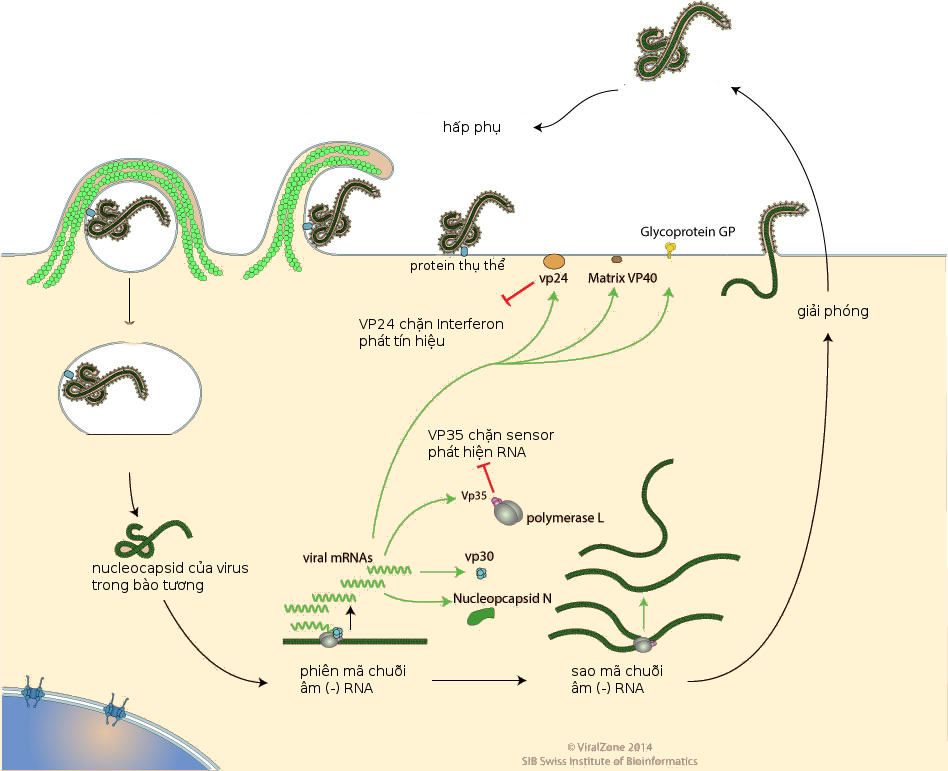
\includegraphics[width=1.0\textwidth,natwidth=610,natheight=642]{Ebolavirus_cycle.png}
		\caption{Vòng đời của \gls{ebov}. Nguồn:http://www.expasy.org/}
		\label{fig:viruscycle}
		\end{figure}
\subsection{Quá trình hệ thống miễn dịch hoạt động}
\hspace{18pt}
		Phân tử \gls{rig-i} có vai trò phát hiện các dsRNA lạ và kích hoạt tế bào sản xuất \gls{ifn}$\alpha / \beta$\cite{Cardenas2006}. Sau khi tế bào bệnh bị phá vỡ do virus nhân lên với số lượng lớn và giải phóng ra ngoài, \gls{ifn}$\alpha / \beta$ cũng được giải phóng theo và bám vào thụ thể của các tế bào lân cận. Sự bám này là tín hiệu cho hệ thống miễn dịch hoạt động và phá hủy tất cả các tế bào có chứa các tác nhân lạ.\cite{DeAndrea2002}
		\begin{figure}[h]
		\centering
		
		\caption{}
		\label{}
		\end{figure}
\subsection{VP35 vô hiệu hệ thống miễn dịch}
\hspace{18pt}
		VP35 bám vào dsRNA của EBOV và không cho \gls{rig-i} phát hiện dsRNA, do \gls{rig-i} phát hiện dsRNA bằng cách liên kết với dsRNA. Theo đó, không có tín hiệu kích hoạt tế bào sản xuất IFN$\alpha / \beta$ và hệ thống miễn dịch không được báo động khi \gls{ebov} phá vỡ thành tế bào và chui ra ngoài\cite{Hartman2004}.
\section{Các phương án ngăn chặn EBOV}

%%%%%%%%%%%%%%%%%%%%%%%%%%%%%%%%%%%%%%%%%%%
%+ Ket thuc Chuong 1.
%%%%%%%%%%%%%%%%%%%%%%%%%%%%%%%%%%%%%%%%%%%


\newpage
\pagestyle{fancy}
%%%%%%%%%%%%%%%%%%%     Chuong 2       %%%%%%%%%%%%%%%%%%%%%%%%
%%%%%%%%%%%%%%%%%%%                    %%%%%%%%%%%%%%%%%%%%%%%%
\setcounter{chapter}{1}
\chapter{Đối tượng và phương pháp nghiên cứu}
\hspace{18pt}
	Khóa luận tập trung nghiên cứu cấu hình 3L25 của phân tử VP35, sử dụng phương pháp \gls{smd} để đánh giá tương tác giữa VP35 và dsRNA
\section{Cấu hình của VP35}
	\subsection{Cấu hình 3L25}
	\hspace{18pt}
		Gồm chuỗi \gls{dsrna} dài 8 đơn vị (8bps) liên kết với 4 phân tử VP35 (chuỗi A, B, C và D). Chuỗi A và B tạo liên kết, với chuỗi B liên kết với đầu chuỗi dsRNA và chuỗi A liên kết với dsRNA dọc theo chiều dài chuỗi. Tương tự với chuỗi C và D. Chuỗi A và C hình thành tương tác Van der Waals với dsRNA. Chuỗi B và D xuất hiện liên kết nhánh phụ trực tiếp với nhóm phosphodiester của dsRNA\cite{Leung2010} (Xem \ref{fig:vp35}).
		\begin{figure}[h]
		\centering
		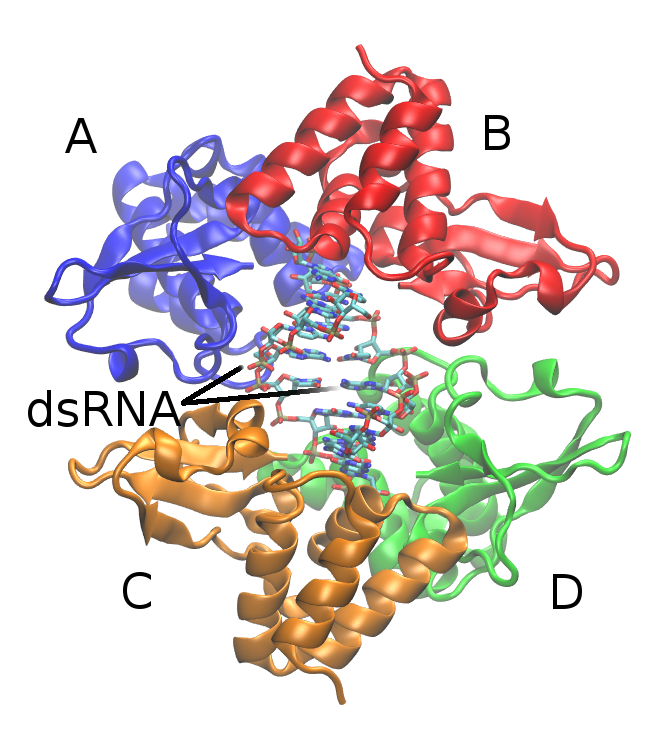
\includegraphics[width=0.7\textwidth,natwidth=610,natheight=642]{VP35.png}
		\caption{4 đơn vị phân tử VP35 bám vào \gls{dsrna} được tô màu xanh dương, đỏ, cam, xanh lá cây.}
		\label{fig:vp35}
		\end{figure}
		Tuy nhiên, để bắt đầu khảo sát cấu trúc 3L25, tôi chọn khảo sát cấu hình chỉ gồm chuỗi A và dsRNA (A-conf), chuỗi B và dsRNA (B-conf), chuỗi A, B và dsRNA (AB-conf).
	\subsection{A-conf}
	\hspace{18pt}
		Gồm chuỗi A và dsRNA. A-conf giúp phân tích tương tác giữa VP35 và dsRNA dọc theo chuỗi (Xem \ref{fig:vp35a}).
		
	\subsection{B-conf}
	\hspace{18pt}
		Gồm chuỗi B và dsRNA. B-conf giúp phân tích tương tác tại đầu chuỗi dsRNA của VP35. Đây là phân tử VP35 tương tác chính với \gls{dsrna} và có vai trò quan trọng trong tương tác giữa hệ các phân tử VP35 và \gls{dsrna}. Xem hình \ref{fig:vp35b}

	\subsection{AB-conf}
	\hspace{18pt}
		Gồm hai chuỗi A và B tương tác với dsRNA (Xem \ref{fig:vp35ab}).
		\begin{figure}[p]
%		\centering
		\begin{subfigure}[h]{0.5\textwidth}
		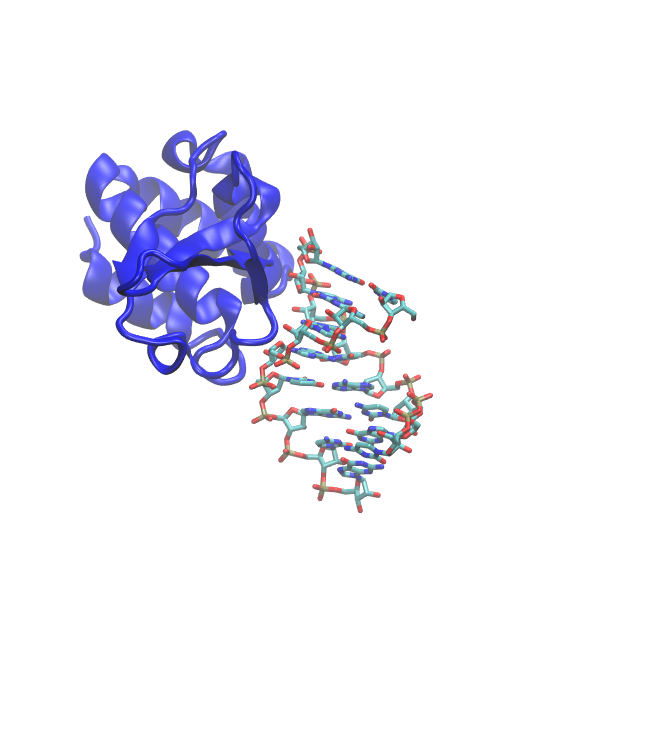
\includegraphics[width=0.9\linewidth,natwidth=610,natheight=642]{VP35_A.png}
		\vspace{-40pt}
		\caption{Chuỗi VP35 A bám vào \gls{dsrna} dài 8bps được tô màu xanh dương.}
		\label{fig:vp35a}
		\end{subfigure}
		\begin{subfigure}[h]{0.5\textwidth}
		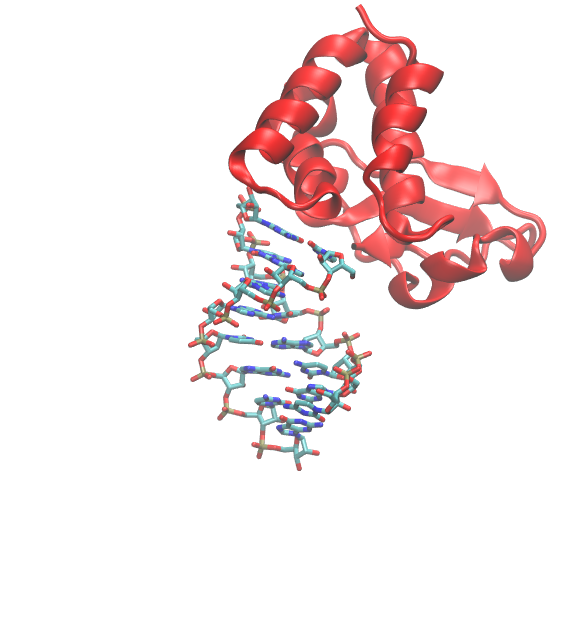
\includegraphics[width=0.9\linewidth,natwidth=610,natheight=642]{VP35_B.png}
		\vspace{-40pt}
		\caption{Chuỗi VP35 B bám vào \gls{dsrna} dài 8bps được tô màu đỏ.}
		\label{fig:vp35b}
		\end{subfigure}
		\\
		\begin{subfigure}[h]{0.9\textwidth}
		\centering
		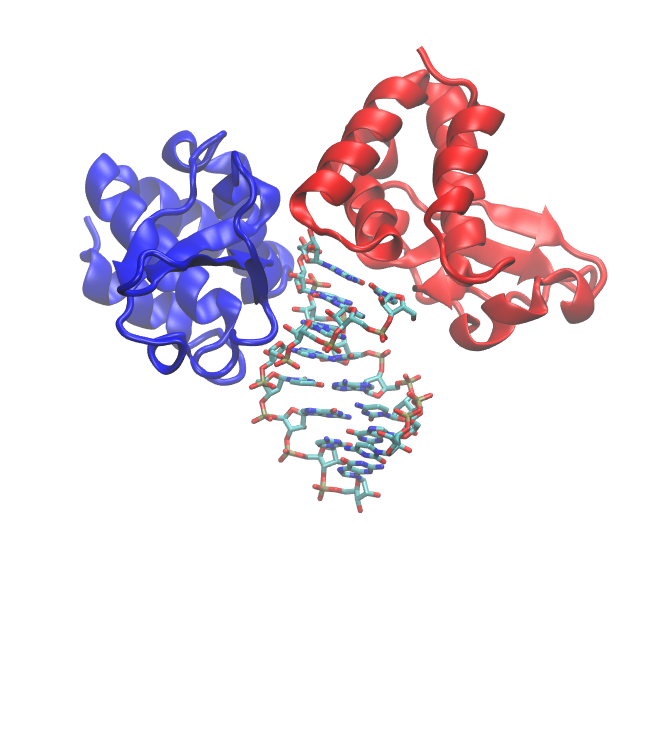
\includegraphics[width=1.0\linewidth,natwidth=610,natheight=642]{VP35_AB.png}
		\vspace{-160pt}
		\caption{2 chuỗi VP35 A và B bám vào \gls{dsrna} dài 8bps được tô màu xanh dương và đỏ.}
		\label{fig:vp35ab}
		\end{subfigure}
		\clearpage

		\caption{Các cấu hình được khảo sát}
		\end{figure}
\newpage
\section{Phương pháp Mô phỏng động học phân tử}
Mô phỏng động lực học phân tử (Molecular Dynamics - MD) là một phương pháp quan trọng giúp tìm hiểu các tính chất vật lý của hệ phân tử sinh học.
	\subsection{Ý tưởng chính}
	\hspace{18pt}
	Khi khảo sát một hệ nhiều hạt, người ta sử dụng các quy luật thống kê do không thể tìm được lời giải giải tích cho mọi tính chất của hệ. Với điều kiện hệ nhiều hạt này tuân theo giả thiết ergodic, việc khảo sát hệ theo thời gian có thể cho ta bức tranh sơ bộ về không gian phase của hệ.
	\Gls{md} cho biết quỹ đạo của từng nguyên tử trong hệ một cách cổ điển, tức là xem mỗi nguyên tử là mô hình một "hạt" tuân theo phương trình chuyển động Newton. Sau khi biết được quỹ đạo theo thời gian, các thông số như vận tốc, động năng, nhiệt độ,... sẽ được tính toán gián tiếp.
%	\subsection{Tham số sử dụng}
	\subsection{Thuật toán Verlet sử dụng trong mô phỏng}
	\hspace{18pt}
		Trong quá trình giải phương trình chuyển động Newton bằng phương pháp số, có một thủ thuật nhằm tính đại lượng tọa độ của hệ hạt với bậc chặt cụt
		Tích phân Verlet\cite{Verlet1967} là một phương pháp số được sử dụng trong phương trình chuyển động Newton. Nó thường dùng để tính quỹ đạo của hạt trong mô phỏng động học và đồ họa máy tính. Thuật toán được phát triển bởi Delambre (1791) và được Verlet sử dụng nhiều trong động học phân tử những năm 60. Nó cũng được dùng để tính toán quỹ đạo sao chổi Halley.
			
		Tích phân Verlet có tính hội tụ cao, có tính chất suy ngược (time-reversible), tính bảo toàn của hệ ngẫu đối của không gian pha và không tốn quá nhiều bước tính so với thuật toán Euler.
			
		Sử dụng khai triển Taylor đến bậc 3 của tọa độ hạt theo thời gian ta được hai phương trình sau:
		\begin{align}
		\vec{x}\left(t+\Delta t\right) &=\vec{x}\left(t\right)+\vec{v}\left(t\right)\Delta t + \dfrac{\vec{a}\left(t\right)\Delta t^{2}}{2} + \dfrac{\vec{b}\left(t\right)\Delta t^{3}}{6} + \mathcal{O}\left(\Delta t^{4}\right)\\
		\vec{x}\left(t-\Delta t\right) &=\vec{x}\left(t\right)-\vec{v}\left(t\right)\Delta t + \dfrac{\vec{a}\left(t\right)\Delta t^{2}}{2} - \dfrac{\vec{b}\left(t\right)\Delta t^{3}}{6} + \mathcal{O}\left(\Delta t^{4}\right)
		\label{verlet1}
		\end{align}
		Cộng hai vế hai phương trình trên, rút ra được:
		\begin{equation}
		\vec{x}\left(t+\Delta t\right)=2\vec{x}\left(t\right)-\vec{x}\left(t-\Delta t\right)+\vec{a}\left(t\right)\Delta t^{2}+\mathcal{O}\left(\Delta t^{4}\right)
		\label{verlet2}
		\end{equation}
		Từ phương trình \eqref{verlet2}, có thể thấy rằng tích phân Verlet đem lại bậc sai số cao hơn nhiều so với phương pháp Euler.
	\subsection{V-rescale và Nosé-Hoover thermostat}
	\hspace{18pt}
		sdf
	\subsection{}
	\subsection{\glsentrytext{amber}}
	\hspace{18pt}
		Tuy có tên gọi là "trường lực" nhưng nó không phải là đại lượng có thứ nguyên của lực. Trường lực (force field - ff) chính là hàm thế năng tương tác giữa các phân tử trong hóa học và sinh học tính toán. Sử dụng gần đúng cổ điển, người ta thường bỏ qua các ảnh hưởng gây ra bởi chuyển động của electron và xét năng lượng của hệ nguyên tử như hàm của các "hạt". Có rất nhiều ff được xây dựng. Trường lực thường xuyên được sử dụng nhất được mang tên AMBER\cite{Duan2003,Cornell1995,Hornak2006}, GROMOS\cite{}, CHARMM\cite{}, OPLS\cite{}. Với mỗi trường lực được phát triển còn có nhiều phiên bản khác nhau với mỗi ưu điểm riêng.
		Khóa luận đã sử dụng phiên bản \gls{amber} để mô phỏng tương tác giữa các phân tử vì đây là trường lực có rất nhiều ưu điểm trong việc mô tả hệ protein-RNA\cite{}. \Gls{amber} có đầy đủ tham số tương tác cho các nguyên tử trong phân tử RNA, protein, kể cả hydro không phân cực. Trong khi đó các trường lực united-atom xem các nguyên tử Hydro và Carbon trong mỗi methyl terminal và mỗi methylene bridge như một điểm tương tác duy nhất. Để mô phỏng thời gian dài, các ff thô (coarse-grained) được sử dụng.
		\Gls{amber} được mô tả bởi một hàm thế như sau:
%		\begin{equation}
		\begin{align}
		V(r^{N}) =& \sum_{ij}^{bond}k_{ij}\left(r_{ij} - r_{ij}^{0}\right)^{2} +\sum_{ijkl}^{dihedrals}k_{ijkl}\left[1+\cos\left(n_{ijkl}\phi_{ijkl}-\phi_{ijkl}^{0}\right)\right] +\nonumber\\
			&+ \sum_{ijkl}^{improper}\frac{1}{2} k_{\xi}\left[\xi_{ijkl}-\xi_{ijkl}^{0}\right]^{2} + \sum_{ijk}^{angles}k_{a}(\theta_{ijk}-\theta_{ijk}^{0})^{2}+ \sum_{ij}\left[\dfrac{q_{i} q_{j}}{\epsilon r_{ij}}+\dfrac{A_{ij}}{r_{ij}^{12}}-\dfrac{B_{ij}}{r_{ij}^{6}}\right]
		\label{ff}
		\end{align}
%		\end{equation}
		Bốn tổng đầu (bốn tổng liên kết - bonded), lần lượt được lấy tổng theo:
		\begin{itemize}
		\item tất cả các liên kết trực tiếp (tương tác 1-2, xem hình \ref{})
		\item tất cả các góc (tương tác 1-3, xem hình \ref{})
		\item tất cả các góc nhị diện (tương tác 1-4, xem hình \ref{})
		\item tất cả các impropers (tương tác 1-4, xem hình \ref{})
		\end{itemize}
		Trong đó, tông liên kết trực tiếp và các số hạng góc được biểu diễn như các dao động tử điều hòa đơn giản. Hai nguyên tử xem như dao động quanh một vị trí cân bằng.
		Các đại lượng $k_{ij}$,$r^{0}_{ij}$,$r_{ij}$ lần lượt là hệ số đàn hồi, độ dài liên kết ở vị trí cân bằng và độ dài liên kết thực tế giữa hai nguyên tử có liên kết hóa trị với nhau $i$ và $j$.
		Trong tổng theo các góc, $k_{ijk}$, $\theta^{0}_{ijk}$, $\theta_{ijk}$, lần lượt là hệ số đàn hồi, góc cân bằng và góc thực tế tạo bởi các nguyên tử $i$, $j$, $k$.
			
		Trong tổng theo góc nhị diện, $k_{ijkl}$, $\phi^{0}_{ijkl}$, $\phi_{ijkl}$ lần lượt là hằng số lực góc nhị diện, góc nhị diện cân bằng và góc nhị diện thực tế tạo bởi các nguyên tử $i$, $j$, $k$, $l$. Hệ số $n_{ijkl}$ là hằng số đối xưng nhận giá trị 1, 2 hoặc 3 ứng với số vị trí cực tiểu khi cho góc nhị diện quay một góc $360^{0}$.
			
		Tương tự, trong tổng theo các impropers, $k_{\xi}$, $\xi^{0}_{ijkl}$, $\xi_{ijkl}$ lần lượt là hằng số lực improper, góc improper cân bằng và góc improper thực tế tạo bởi các nguyên tử $i$, $j$, $k$, $l$.
			
		Các tổng cuối trong phương trình \eqref{ff} là các tổng không liên kết (non-bonded). Các tổng này bao gồm tương tác Van der Waals (hình \ref{}) và tương tác tĩnh điện (hình \ref{}). Tương tác Van der Waals được mô tả bởi thế Lennard-Jones (6-12) và tương tác tĩnh điện được mô tả bởi thế Coulomb với giả thiết là điện tích điểm nằm tại tâm của nguyên tử \cite{}. Hằng số điện môi $\epsilon$ đặc trưng cho môi trường giữa hai nguyên tử, tham số $B_{ij}$ và $A_{ij}$ là các tham số 6-12 đặc trưng cho từng nguyên tố.
			
		Tất cả các hằng số lực, các tham số ứng với tọa độ cân bằng, các tham số 6-12 và hệ số đối xứng $n_{ijkl}$ được dẫn ra từ các tính toán lượng tử với độ chính xác cao và từ thực nghiệm\cite{}.
\section{\glsentryfull{smd}}
Chính là \gls{md} nhưng đặt thế năng thay đổi theo thời gian lên các nhóm phân tử xác định để tách các nhóm này ra. Có hai cách xác định tham số của thế năng, tương ứng với hai cách "kéo" các nhóm phân tử ra: kéo với lực kéo không đổi hoặc kéo nhóm tách ra với vận tốc không đổi. Đề tài sử dụng phương pháp kéo với vận tốc không đổi.
Trong suốt quá trình kéo, dễ dàng để tính toán lực kéo các nhóm. Từ đó phác thảo được tương tác giữa các nhóm phân tử.
\section{Các công cụ phân tích kết quả}
	\subsection{Lực kéo tối đa}
	\hspace{18pt}
	Là lực lớn nhất dùng để kéo hai phân tử ra trong suốt quá trình mô phỏng. Do hệ phân tử đã ở vị trí ứng với đáy của giếng thế địa phương, nên để tách hai nhóm phân tử protein và \gls{dsrna} ra thì lực dùng để tách hai nhóm ra sẽ lớn dần đến một giá trị mà tại đó hai nhóm không còn tương tác đáng kể với nhau nữa.
	Việc so sánh lực kéo tối đa giữa các
	\subsection{Liên kết Hydro}
	\hspace{18pt}
	Liên kết Hydro (H-bond) là liên kết vật lý đóng góp chủ yếu trong tương tác giữa hai nguyên tử\cite{}
	Liên kết Hydro là liên kết giữa nguyên tử phân cực dương (donor) và nguyên tử phân cực âm (acceptor) thỏa điều kiện (i) cách nhau một khoảng 3\={A} và (ii) góc nhị diện tạo bởi donor và acceptor là lớn hơn hoặc bằng $120^{0}$.


%%%%%%%%%%%%%%%%%%%%%%%%%%%%%%%%%%%%%%%%%%%
%+ Ket thuc Chuong 2.
%%%%%%%%%%%%%%%%%%%%%%%%%%%%%%%%%%%%%%%%%%%


\newpage
\pagestyle{fancy}
%%%%%%%%%%%%%%%%%%%     Chuong 3       %%%%%%%%%%%%%%%%%%%%%%%%
%%%%%%%%%%%%%%%%%%%                    %%%%%%%%%%%%%%%%%%%%%%%%
\setcounter{chapter}{2}
\chapter{Kết quả và thảo luận}
%\section{A-conf}
%\hspace{18pt}
\section{B-conf}
Đây là chuỗi VP35 end-cap của \gls{dsrna} (xem hình \ref{fig:vp35b}).
	\begin{figure}[b!]
	\centering
	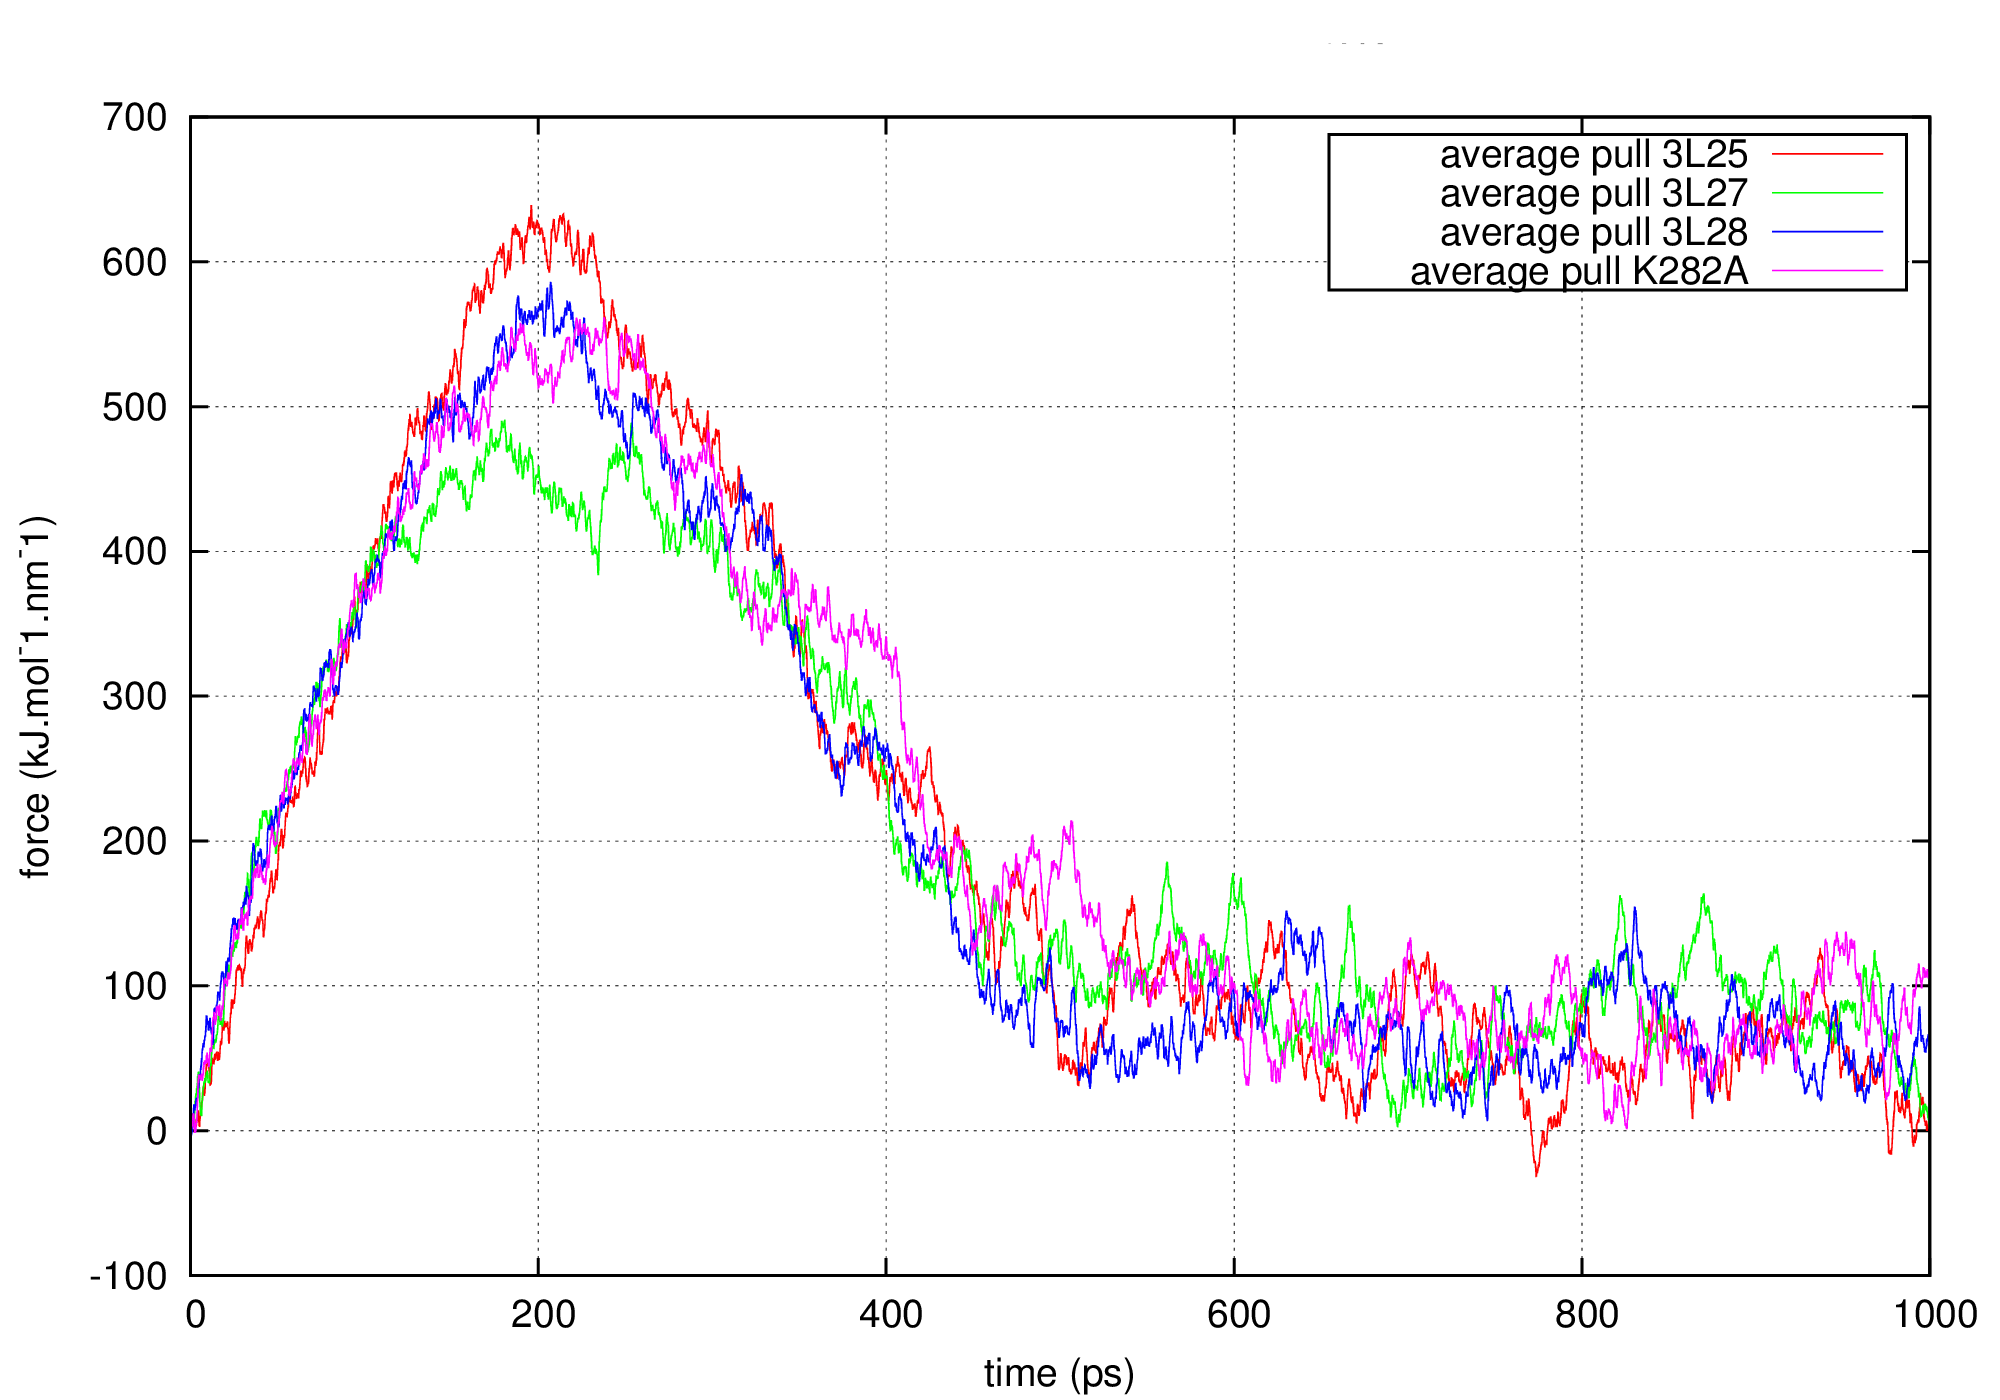
\includegraphics[width=1.0\textwidth,natwidth=610,natheight=642]{pullf}
	\caption{}
	\end{figure}

	\begin{figure}[t]
	\centering
	\includegraphics[height=0.3\textheight,natwidth=610,natheight=642]{../../../Analysis/non_md/3L25/hbond}
	\caption{Tỉ lệ \% liên kết hydro tạo bởi các cặp amino acid và \gls{dsrna}}
	\label{fig:hbond25}
	\end{figure}
	\begin{figure}[p]
	\centering
	\includegraphics[height=0.3\textheight,natwidth=610,natheight=642]{../../../Analysis/non_md/3L27/hbond}
	\caption{Tỉ lệ \% liên kết hydro tạo bởi các cặp amino acid và \gls{dsrna}}
	\label{fig:hbond27}
	\end{figure}
	\begin{figure}[p]
	\centering
	\includegraphics[height=0.3\textheight,natwidth=610,natheight=642]{../../../Analysis/non_md/3L28/hbond}
	\caption{Tỉ lệ \% liên kết hydro tạo bởi các cặp amino acid và \gls{dsrna}}
	\label{fig:hbond28}
	\end{figure}
	\subsection{Phân tử không đột biến}
\hspace{18pt}
	Dựa vào đồ thị lực kéo dùng để tách VP35 khỏi \gls{dsrna} theo thời gian dễ dàng xác định được giá trị lực kéo tối đa. Lực kéo tối đa này cho thấy VP35 chuỗi B gắn khá chặt vào \gls{dsrna} 
	\subsection{Đột biến R312A}
\hspace{18pt}
	\subsection{Đột biến K339A}
\hspace{18pt}
\section{AB-conf}
\hspace{18pt}
%%%%%%%%%%%%%%%%%%%%%%%%%%%%%%%%%%%%%%%%%%%
%+ Ket thuc Chuong 3.
%%%%%%%%%%%%%%%%%%%%%%%%%%%%%%%%%%%%%%%%%%%


\newpage
\pagestyle{fancy}
%%%%%%%%%%%%%%%%%%%     Chuong 4       %%%%%%%%%%%%%%%%%%%%%%%%
%%%%%%%%%%%%%%%%%%%                    %%%%%%%%%%%%%%%%%%%%%%%%
\setcounter{chapter}{3}
chapter{Kết luận và hướng phát triển tiếp theo của đề tài}
\hspace{18pt}
	
	
	Đề tài có nội dung khá ngắn gọn và chưa bao quát hết được các hiện tượng cơ bản khác. Tuy nhiên, phần nào đã thể hiện được tinh thần của mô phỏng trong việc áp dụng vào khoa học. Nếu có thêm thời gian, ắt hẳn đề tài còn có thể mô hình hoá nhiều đối tượng hơn.\\ 
	
%%%%%%%%%%%%%%%%%%%%%%%%%%%%%%%%%%%%%%%%%%%
%+ Ket thuc Chuong 4.
%%%%%%%%%%%%%%%%%%%%%%%%%%%%%%%%%%%%%%%%%%%


%%%%%%%%%%%%%%%%%%%     Bibliography    %%%%%%%%%%%%%%%%%%%%%%%
%%%%%%%%%%%%%%%%%%%                     %%%%%%%%%%%%%%%%%%%%%%%
%\nocite{*}
\printbibliography
\addcontentsline{toc}{chapter}{Tài liệu tham khảo}
\clearpage





%%%%%%%%%%%%%%%%%%%     Appendice       %%%%%%%%%%%%%%%%%%%%%%%
%%%%%%%%%%%%%%%%%%%                     %%%%%%%%%%%%%%%%%%%%%%%
\appendix
\addcontentsline{chapter}{Phụ lục}
\clearpage
\newpage
%%%%%%%%%%%%%%%%%%      Phụ lục       %%%%%%%%%%%%%%%%%%
%%%%%%%%%%%%%%%%%%                    %%%%%%%%%%%%%%%%%%
\chapter{Chương trình GROMACS}
Đây là gói chương trình mã nguồn mở sử dụng giấy phép GPL3 dùng trong đề tài để thực hiện mô phỏng và đánh giá kết quả mô phỏng động học phân tử.

Name:    Interaction Evaluation
Descr:   Calculates interactions for a microstate
Depen:   Bonded int., Non-bonded int.
Input:   Rules, Microstate, Switches
Output:  V, F and/or virial
Req:     Maximum efficiency, will use cache
 
Name:    Bonded/Listed Interaction Evaluation
Descr:   Calculates interactions from a specified list (in the rules)
Depen:  
Input:   Rules, Microstate, Switches
Output:  V, F and/or virial, evaluation count (for checking the total count)
Req:     Maximum efficiency, will use cache (e.g. force tables)
 
Name:    Pair Interaction Evaluation
Descr:   Calculates pair interactions within a cut-off distance
Depen:  
Input:   Rules, Microstate, Switches
Output:  V, F and/or virial
Req:     Maximum efficiency, will use cache (e.g. pair list, force tables)
 
Name:    Virtual Sites
Descr:   Determines virtual site coordinates and redistribution
virtual site của mô hình nước
Input:   Rules, Microstate or F
Output:  Microstate or F
Req:     Could cache coefficients from X calculation for F
 
Name:    Propagation
Descr:   Propagates the microstate with several MD, EM or MC propagators
Depen:   Constraints
Input:   Microstate, F, T, P, Hamiltonian state, external fields
Output:  V, F and/or virial
Req:     Should support several integrators using a few hooks
 
Name:    Constraints
Descr:   Applies contraints to unconstrained X, V or F
Depen:  
Input:   Rules, Microstate and possibly F
Output:  Constrained (or constraint components of) X, V or F
Req:     Must be able to work in parallel with MPI and/or threads
 
Name:    Measurements
Descr:   Handles measurements during simulation
Depen:   I/O
Input:   Microstate, Energies, ...
Output:  Energy file, Log
Req:     Also records history which needs to be stored in checkpoint
 
Name:    Energy Reduction (separate from Measurements?)
Descr:   Reduce local energy terms over MPI processes (and threads?)
Depen:  
Input:   Local energies
Output:  Global energies
Req:    
 
Name:    Domain Decomposition
Descr:   Decomposes the system over domains and handles communication
Depen:  
Input:   Global Rules, Global Microstate, Parallel system setup
Output:  Local Rules, Local Microstate
Req:    
 
Name:  COM calculation
Descr:  Calculates center of mass(es) of group(s) of particles
Depen:
Input:  Coordinate and mass vector distributed over processes/threads, group(s)
Output: COM(s) on each thread/process
Req:

\subsection{Flow chart of the program}
\tikzstyle{startstop} = [rectangle, rounded corners, minimum width=3cm, minimum height=1cm,text centered, draw=black, fill=white, thick]
\tikzstyle{io} = [trapezium, trapezium left angle=70, trapezium right angle=110, minimum width=3cm, minimum height=1cm, text centered, text width=6cm, draw=black, fill=white, thick]
\tikzstyle{process} = [rectangle, minimum width=3cm, minimum height=1cm, text centered,text width=4cm, draw=black, fill=white, thick]
\tikzstyle{decision} = [diamond, minimum width=3cm, minimum height=1cm, text centered, draw=black, fill=white, thick]
\tikzstyle{arrow} = [thick,->,>=stealth]
\begin{figure}[H]
\begin{center}
	\begin{tikzpicture}[node distance=2cm]
	\node (start) [startstop] {Start};
	\node (in1) [io, below of=start,yshift=-0.2cm] {Input \par Incident energy \par Target, projectile's mass, spin \par $l\kk{max}$};
	\node (pro1) [process, below of=in1,yshift=-0.7cm] {Calculate: $k\kk{dA}, k\kk{dA}, k\kk{dA}, R$ \par $ l=l\kk{min}$};
	\node (pro2) [process, below of=pro1, yshift=-0.0cm] {$\theta\kk{max}=180, \theta=1$};
	\node (pro3) [process, below of=pro2, yshift=+0.4cm] {$ \left( \dfrac{\text{d}\sigma}{\text{d}\Omega} \right) $};
	\node (pro4) [process, below of=pro3, yshift=+0.4cm] {$\theta= \theta+\Delta\theta $};
	\node (dec1) [decision, below of=pro4, yshift=-0.3cm] {$\theta \leqslant \theta\kk{max}$};
	\node (pro5) [process, below of=dec1, yshift=-0.3cm] {$l=l+2$};
	\node (dec2) [decision, below of=pro5, yshift=-0.3cm] {$l \leqslant l\kk{max}$};
	%\node (out1) [io, below of=dec2,yshift=-0.1cm] {Output};
	\node (stop) [startstop, below of=dec2,yshift=-0.3cm] {Output};
	\node [coordinate, below left =1cm and 1cm of pro5] (left2) {};  
	\node [coordinate, below left =1cm and 1cm of pro3] (left1) {}; 
	\node [coordinate, right =1cm of pro3] (right2) {};    
	
	\draw [arrow] (start) -- (in1);
	\draw [arrow] (in1) -- (pro1);
	\draw [arrow] (pro1) -- (pro2);
	\draw [arrow] (pro2) -- (pro3);
	\draw [arrow] (pro3) -- (pro4);
	\draw [arrow] (pro4) -- (dec1);
	\draw [arrow] (dec1) -- node[anchor=west] {no} (pro5);
	\draw [arrow] (dec1) -| node[anchor=west] {yes} (right2) |- (pro3);
	\draw [arrow] (pro5) -- (dec2);
	\draw [arrow] (dec2) -| node[anchor=east] {yes} (left2) -- (left1) |- (pro2);
	\draw [arrow] (dec2) -- node[anchor=west] {no}(stop);
	%\draw [arrow] (out1) -- (stop);
	\end{tikzpicture}
	\caption{Flow chart of the code}
\end{center}
\end{figure}
Add /home/quyngan/.texlive/2014/texmf-dist/doc/man to MANPATH.
Add /home/quyngan/.texlive/2014/texmf-dist/doc/info to INFOPATH.
Most importantly, add /home/quyngan/.texlive/2014/bin/x86_64-linux
to your PATH for current and future sessions.
\end{document}
